\documentclass[11pt]{article}

\usepackage{algorithmic}
\usepackage{amsmath}
\usepackage{graphicx}
\usepackage{hyperref}
\usepackage{fancyhdr}


\renewcommand{\baselinestretch}{1.2}
\setlength{\topmargin}{-0.5in}
\setlength{\textwidth}{6.5in}
\setlength{\oddsidemargin}{0.0in}
\setlength{\textheight}{9.1in}

\fancyhfoffset{0in}

\newlength{\pagewidth}
\setlength{\pagewidth}{6.5in}
\pagestyle{empty}

\def\pp{\par\noindent}

\special{papersize=8.5in,11in}

\author{Junwei Jason Zhang \\Jian Jiang\\ Daniel Guo}
\title{Mid-report of CV Project\\Efficient MRF Deformation Model for Non-Rigid Image Matching}
\begin{document}
\maketitle

\section{Algorithm Pipeline}
\begin{itemize}
    \item
    \textbf{Input} Two images, one of which is the template image and the other is the target. The target image could be any form of the following three deformations(Figure 1).
        \begin{itemize}
            \item Rotation + Scaling
            \item Twirl
            \item Twirl + Projective
        \end{itemize}
    \item 
    \textbf{Output} A non-rigid deformation transforming the area of interest from template image to target image
    \item
    \textbf{Crop} out the area of interest from the template image
    \item
    \textbf{Block Model} Cut the template graph into blocks with size of $4\times 4$
    \item
    \textbf{Compute deformation} which transforms each block in template to its corresponding block in target
    \item
    \textbf{Reconstruct} the corresponding block region in target image
\end{itemize}
\begin{figure}[!htp]
    \centering
    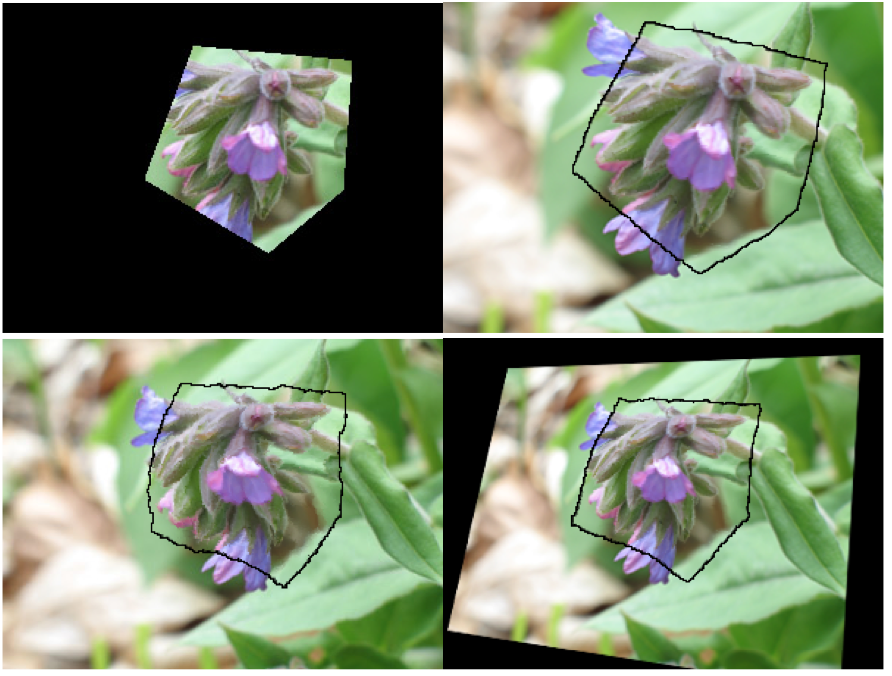
\includegraphics[scale = 0.7]{midreport.png}
    \caption{Three kinds of deformations}
\end{figure}
\section{MRF energy function}
The criterion of computing the corresponding block is to minimize the energy 
\begin{equation}
E(x|\theta ) = \sum_{s \in V} \theta_s (x_s)+ \sum_{st \in E} \theta_{st} (x_s,x_t)
\end{equation}
Where $x_s, x_t$ is the labels for each block accounting for the translation. $\theta_s(x_s)$ here is the data term, which is reponsible for the similarity of some specific pixel in the template image and the corresponding pixel in the target image. $\theta_{st} (x_s, x_t)$ here is the pairwise term, which accounts for the similarity of neighbouring pixels in one image. Shown in Figure 2.
\begin{figure}[!htp]
    \centering
    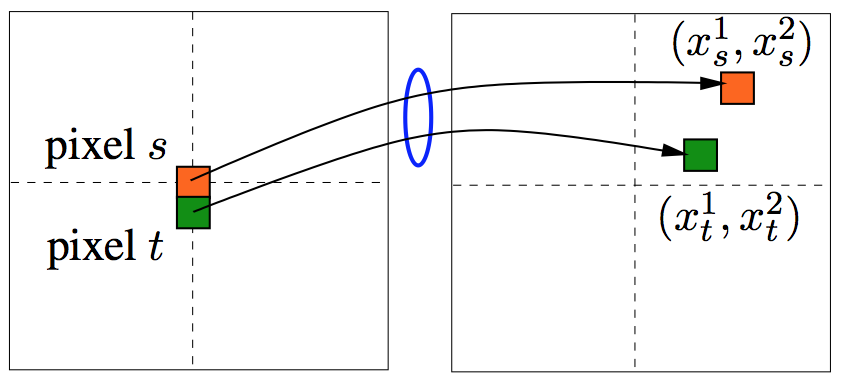
\includegraphics[scale=0.8]{midreport2.png}
    \caption{Data term and Pairwise term}
\end{figure}
\subsection{Decomposed Model}
We decompose the definition of the data term and pairwise term into two layers, one of which accounts for the translation in $x$ direction, and the other accounting for the translation in $y$ direction, which is shown in Figure 3.
        \begin{figure}[!htp]
            \centering
            \includegraphics[scale=0.8]{7.png}
            \caption{Two-layers Model}
        \end{figure}
Thus, the definition of the two terms are
\begin{equation}
    \theta_{st}(x_s, x_t) = \frac{I_s^1 - I_{s+(x_s, x_t)}^2}{2\sigma_I^2},\ s\in V^1,\ t\in V^2,\ st \in E^{12}
\end{equation}
\begin{equation}
    \theta_{st}(x_s, x_t) = \frac{(x_s - x_t)^2}{2\sigma_{x}^2},\ st\in E^{i}\ i = 1,2
\end{equation}

\end{document}


